
%\documentclass[12pt]{report}

\documentclass[12pt]{article}
%\usepackage{natbib}  % used for citations
\usepackage[parfill]{parskip} %used for formatting style of text



\usepackage{graphicx,fancyhdr}
\usepackage{amssymb,amsmath}
\usepackage{epigraph,fancyvrb,eqparbox}
\usepackage[multiple]{footmisc}
\usepackage{menukeys}
\usepackage{menukeys}
\usepackage{url}
\usepackage[colorlinks = true, linkcolor = blue, urlcolor = blue]{hyperref}
\usepackage{setspace}

\pagestyle{fancyplain}

%\usepackage{hyperref}
%\usepackage{epsf,psfig,graphicx,fancyheadings}
% \textwidth 7in
% \textheight 9in
% \oddsidemargin 0in
% \topmargin -.25in

%-----------------------------------------------
% The following settings are from Dr. Davidian's
% ST810A Handout on Advanced LaTeX Features

%\setlength{\paperheight}{11.0in}
%\setlength{\paperwidth}{8.5in}

%%%%%%%%%%%%%%%%%%%%%%%%%%%%%%%%%%%%%%%%%%%%%%%%%
% For Desktop @ CalPoly (for Postscript)

%\setlength{\oddsidemargin}{0.5in}
%\setlength{\evensidemargin}{0.5in}
%\setlength{\topmargin}{-.5in}

%%%%%%%%%%%%%%%%%%%%%%%%%%%%%%%%%%%%%%%%%%%%%%%%%
% For Laptop @ Calpoly (for Postscript)

% \setlength{\oddsidemargin}{0.in}
% \setlength{\evensidemargin}{0.in}
% \setlength{\topmargin}{0.25in}

%%%%%%%%%%%%%%%%%%%%%%%%%%%%%%%%%%%%%%%%%%%%%%%%%
% For Desktop @ CalPoly (for PDF)

%\setlength{\oddsidemargin}{0.in}
%\setlength{\evensidemargin}{0.in}
%\setlength{\topmargin}{-.5in}
%
%%%%%%%%%%%%%%%%%%%%%%%%%%%%%%%%%%%%%%%%%%%%%%%%%%
%% For Laptop @ Calpoly (for PDF)
%
%% \setlength{\oddsidemargin}{0.in}
%% \setlength{\evensidemargin}{0.in}
%% \setlength{\topmargin}{0.25in}
%
%
%
%\setlength{\oddsidemargin}{0.0in}
%\setlength{\topmargin}{-0.5in}
%\setlength{\headheight}{0.20in}
%\setlength{\headsep}{3ex}
%\setlength{\baselineskip}{2ex}
%\setlength{\textheight}{9in}
%\setlength{\textwidth}{6.4in}
%\renewcommand{\baselinestretch}{1.1}

% Sets margins to 1 in
\addtolength{\oddsidemargin}{-.5in}%
\addtolength{\evensidemargin}{-.5in}%
\addtolength{\textwidth}{1in}%
\addtolength{\textheight}{1.3in}%
\addtolength{\topmargin}{-.8in}%

%\setlength{\headheight}{0.20in}
%\setlength{\headsep}{3ex}
%\setlength{\headrulewidth}{0.2pt}
%\setlength{\footrulewidth}{0.15pt}
%\setlength{\parskip}{2.3ex}
% %set to no indentation
%\setlength{\parindent}{0.0in}
%\setlength{\baselineskip}{2ex}
%\setlength{\textheight}{9.in}
%\setlength{\textwidth}{6.5in}

\def \doublespace{\openup 2\jot}
% For double or 1.5 spacing
%\renewcommand{\baselinestretch}{1.5}
\tolerance=500

\def\boxit#1{\vbox{\hrule\hbox{\vrule\kern6pt
\vbox{\kern6pt#1\kern6pt}\kern6pt\vrule}\hrule}}
\renewcommand{\theequation}{\thesection.\arabic{equation}}
% The following for TOC
%\renewcommand{\thepage}{\roman{page}}
% to be followed by this for the main text
\renewcommand{\thepage}{\arabic{page}}


%-----------------------------------------------

%%%%%%%%%%%%%%%%%%%%%%%%%%%%%%%%%%%%%%
%Define any shortcut aliases below

\newtheorem{theo}{Theorem}[section]

\newenvironment{note}{\begin{quote}\emph{Note:\ }}{\end{quote}}
\newenvironment{defn}{
\begin{description}
\item[Definition ]}
{\end{description}}

\newenvironment{ttscript}[1]{%
    \begin{list}{}{%
    \settowidth{\labelwidth}{\texttt{#1}}
    \setlength{\leftmargin}{\labelwidth}
    \addtolength{\leftmargin}{\labelsep}
    \setlength{\parsep}{0.5ex plus0.2ex minus0.2ex}
    \setlength{\itemsep}{0.3ex}
    \renewcommand{\makelabel}[1]{\texttt{##1\hfill}}}}
    {\end{list}}

\newcommand{\bt}{\begin{tabular}}
\newcommand{\et}{\end{tabular}}
\newcommand{\bc}{\begin{center}}
\newcommand{\ec}{\end{center}}
\newcommand{\bi}{\begin{itemize}}
\newcommand{\ei}{\end{itemize}}
\newcommand{\be}{\begin{enumerate}}
\newcommand{\ee}{\end{enumerate}}
\newcommand{\bq}{\begin{quote}}
\newcommand{\eq}{\end{quote}}
\newcommand{\vect}[1]{\mbox{\boldmath $ #1$}}
\newcommand{\avg}[1]{$\overline{#1}$}
\newcommand{\bmp}{\begin{minipage}}
\newcommand{\emp}{\end{minipage}}
\newcommand{\hr}{\u{\hspace{7in}}}
\newcommand{\sr}{\u{\hspace{5in}}}
\newcommand{\chs}{\chi^2}

\newcommand{\labn}[1]{\Large{\textbf{\fbox{Lab #1}}}\hspace{0.1in} \normalsize{\emph{Some of these problems may be more challenging than others. Please feel free to work with others, attend office hours, or post on the course discussion forum if you need help.  While collaboration with other students is encouraged, each student is responsible for submitting his or her own work.  This assignment should be submitted in one well-commented SAS program.  For any questions that require a written answer, do so in the SAS comments.  Be sure to re-name the uploaded SAS scripts according to the naming convention}} \texttt{LastnameFirstinitial\textunderscore Lab\#.sas} (\emph{e.g.,} \texttt{PileggiS\textunderscore Lab#1.sas}).}


\newcommand{\hd}[1]{\lhead{STAT 330/530: Lab #1}\rhead{Pileggi, FA17}}
\newcommand{\bs}{\underline{\hspace{0.5in}}}

%\newcommand{\bv}{\footnotesize
%\bmp{.5\textwidth}
%\begin{Verbatim}[frame=single,label=SAS Code,commandchars=\\\{\}],xrightmargin=.5\textwidth}
%
%\newcommand{\ev}{\end{Verbatim}
%\emp
%\normalsize}

\newcommand{\bv}{\begin{code}}
\newcommand{\ev}{\end{code}}

 \newenvironment{code}[1]%
  {\vspace{.1in}\footnotesize\Verbatim[frame=single,label=SAS Code,commandchars=\\\{\},xrightmargin=#1\textwidth,framesep=.2in,labelposition=all]}
  {\endVerbatim\normalsize}

\newenvironment{craw}[2]%
{\vspace{.1in}\footnotesize\Verbatim[frame=single,label=#2,commandchars=\\\{\},xrightmargin=#1\textwidth,framesep=.2in,labelposition=all]}
  {\endVerbatim\normalsize}

\newenvironment{cbox}[1]%
{\vspace{.1in}\footnotesize\Verbatim[frame=single,commandchars=\\\{\},xrightmargin=#1\textwidth,framesep=.2in,labelposition=all]}
  {\endVerbatim\normalsize}

\newcommand{\head}[1]{\large \textbf{#1} \normalsize}

\newcommand{\ttt}[1]{\textbf{\texttt{#1}}}


\newcommand{\bsval}[1]{\underline{\hspace{0.2in}{[#1]}\hspace{0.2in}}}

\newcommand{\ttb}{\textbf}
\newcommand{\tte}{\emph}
\newcommand{\ttu}{\underline}



\newcommand{\jdhr}{\vspace{0.2in}\hrule}


\newcommand{\uspace}[1]{\underline{\hspace{#1}}}

\newenvironment{ident}{\begin{list}{}{}
         \item[]}{\end{list}}

\newenvironment{proposition}{
\begin{description}
\item[Proposition: ]}
{\end{description}}

\newcommand{\bpr}{\begin{proposition}}
\newcommand{\epr}{\end{proposition}}



% \newenvironment{example}
%     {
%         \begin{list}{\textbf{Example:}}
%         {
%         \settowidth{\labelwidth}{}
%         \setlength{\leftmargin}{\labelwidth}
%         }
%     }
%     {\end{list}}


\newenvironment{example}{
\jdhr \vspace{-.17in}\jdhr
\textbf{Example: }}
{}

\newcommand{\bex}{\begin{example}}
\newcommand{\eex}{\end{example}}

\newenvironment{onyourown}{
\jdhr \vspace{-.17in}\jdhr
\textbf{On Your Own: }}
{}

\newcommand{\boy}{\begin{onyourown}}
\newcommand{\eoy}{\end{onyourown}}


%\newenvironment{debug}{
%\jdhr \vspace{-.17in}\jdhr
%\ttb{Debug the Code}
%\fbox{
%\bmp{.95in}
%\includegraphics[height=.35in]{C:/images/bug4.jpg}\includegraphics[height=.35in]{C:/images/buggy8.jpg}
%\emp}
%}
%{\jdhr}

\newenvironment{debug}{
\jdhr \vspace{-.17in}\jdhr
\ttb{Debug the Code: }
\fbox{
\bmp{.95in}
\includegraphics[height=.35in]{C:/images/bug4.jpg}\includegraphics[height=.35in]{C:/images/mushi90.jpg}
\emp}
}
{}


\newcommand{\bbug}{\begin{debug}}
\newcommand{\ebug}{\end{debug}}


\begingroup
  \catcode `_=11
  \gdef\myuscore{_}
  \catcode `~=11
  \gdef\mytilde{~}
  \catcode `\|=0
  \catcode `\\=11
  |gdef|mybs{\}
|endgroup

%Define any shortcut aliases above


%....................................................................
%....................................................................
%....................................................................
%....................................................................
%....................................................................
%....................................................................
%....................................................................
%....................................................................



\usepackage{amssymb}
				




\begin{document}
\hd{10}
\labn{10}
\vskip10pt

Many people incur debt at some point in their life, and for some it starts with student loans. The \texttt{studentloans} data is for students at some of the most and least expensive private institutions.\\
\vskip10pt
{\renewcommand{\arraystretch}{1.5}
\begin{tabular}{p{3cm} | p{12cm}}
\ttt{Loan} &  the total amount that the student took out in loans - the loan does not accrue interest until after the student graduates \\
\ttt{Interest} & the rate is the \emph{annual} rate which the amount to be paid back increases after graduation, and is compounded \emph{monthly} (so the monthly interest is \ttt{Interest/12})\\
\ttt{College\textunderscore Start} &  the year the student started college\\
\ttt{Years}&  the total number of years the student spent in school\\
\ttt{Salary} &  the current salary of these former students\\
\ttt{Payment} & the \emph{monthly} payment the student is making towards the loan, after graduation\\
\end{tabular}}

\begin{enumerate}
\item Create a library reference called \texttt{mylib} to access the \texttt{studentloans} and \texttt{adni} SAS data sets.
\item Assuming fixed income and payments, determine when each person pays off their loan by completing the following tasks with the \texttt{studentloans} data set.
        \begin{enumerate}
        \item Write a loop that identifies how many months until the loan is paid off (i.e., the balance is $\leq 0$).  Here is the idea behind the calculations:
        \begin{itemize}
            \item initialize the values of 
            \begin{itemize} 
            \item \texttt{months} to 1
            \item \texttt{balance} to \texttt{loan} 
            \item \texttt{monthly\_interest} to \texttt{interest/12}
            \end{itemize}
            \item each month, the monthly payment is deducted from the loan balance
            \item each month, the loan balance increases by the interest rate
            \item increment months by one
            \item continue until the loan balance is less than zero
        \end{itemize}
        \item Print your output with an appropriate title.  Your results should look something like this (only select variables shown):
        \item[] 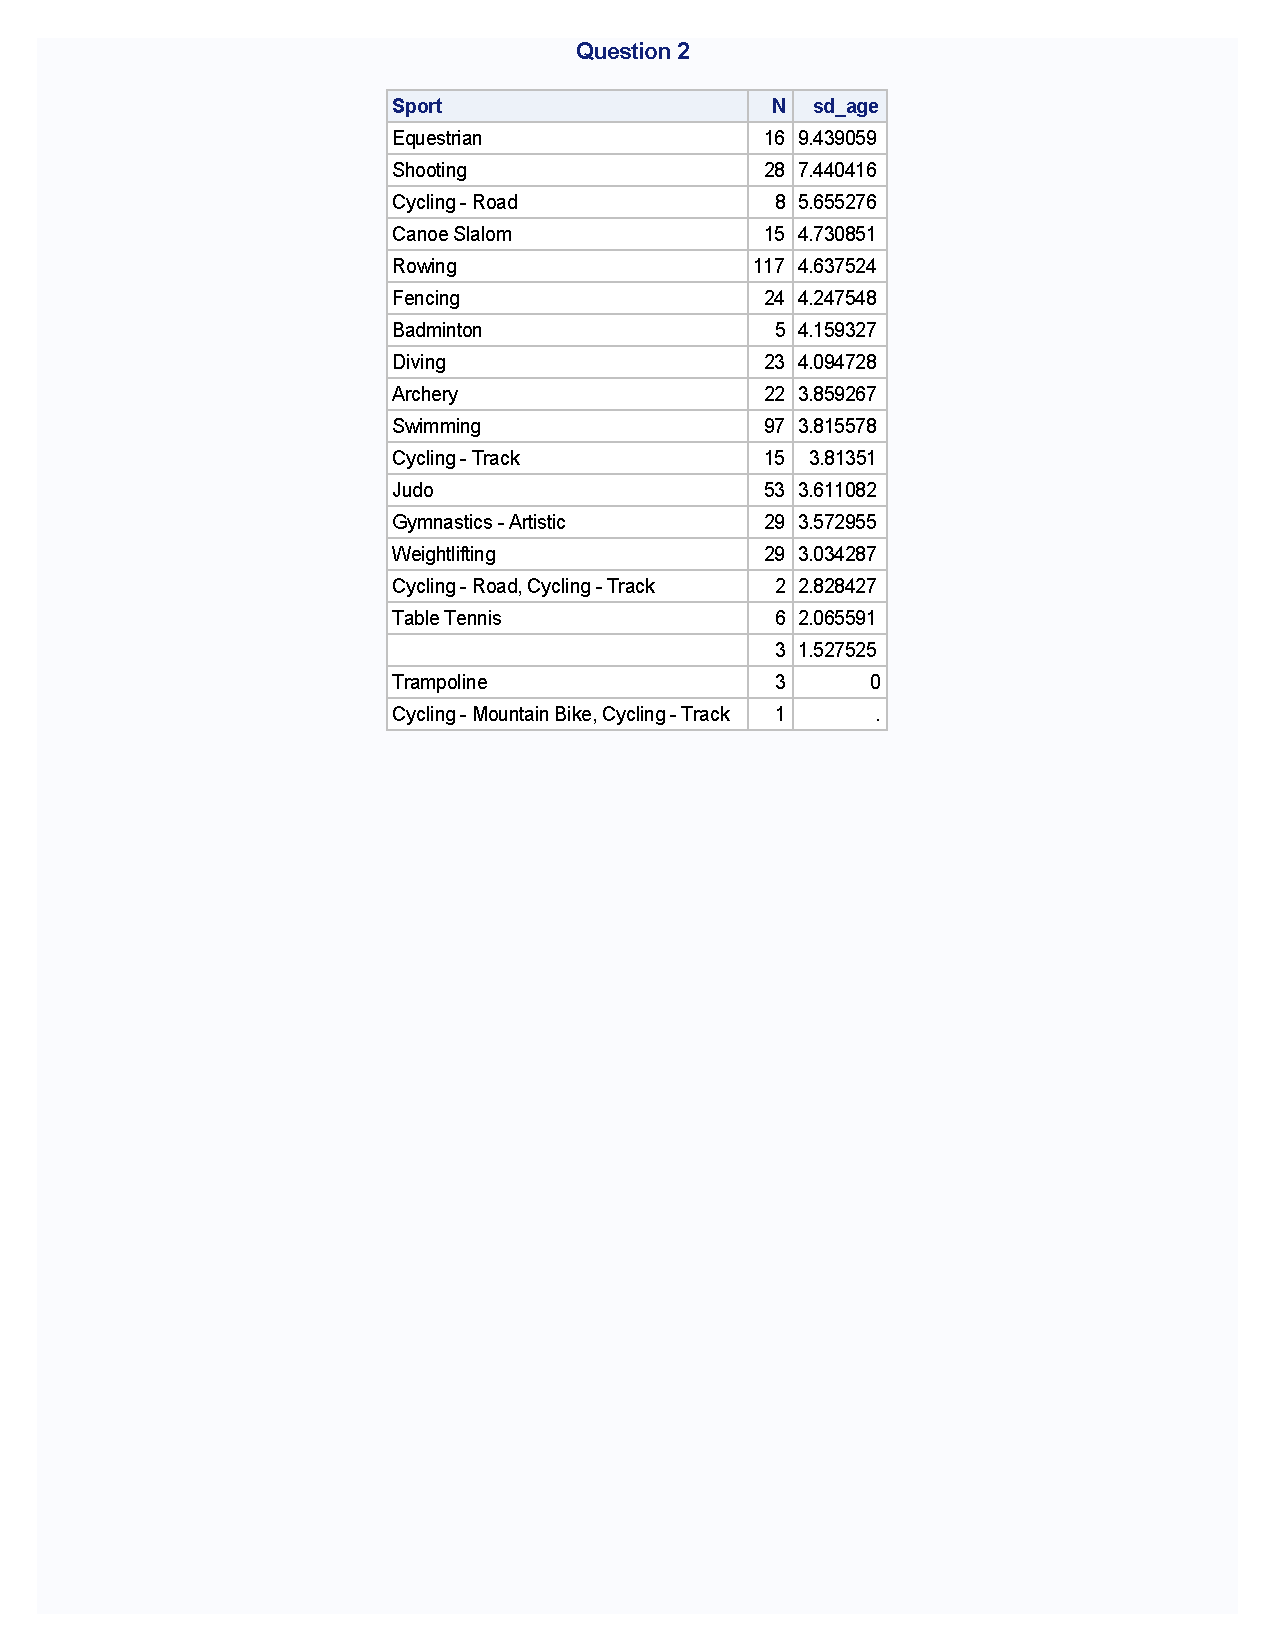
\includegraphics[trim=7cm 22cm 7cm 1.5cm,clip]{q2.pdf}
        \item In a comment in your SAS code, briefly describe how SAS executed this data step.
        \item[]
        \end{enumerate}
\end{enumerate}
Recall the \ttt{adni} data set from the Alzheimer's Disease Neuroimaging Initiative (ADNI) longitudinal study that began in 2005.  This research is designed to track AD biomarkers, identify at-risk patients, and evaluate the efficacy of novel treatments. 
\vskip20pt
\begin{tabular}{r|l}
\ttt{DX}   &  Alzheimer's disease diagnosis\\
           & \hspace{0.2in} 1 - Normal cognitive function\\
           & \hspace{0.2in} 2 - Mild cognitive impairment (MCI) \\
           & \hspace{0.2in} 3 - Alzheimer's disease (AD) \\
\ttt{AGE} &  Age (years) \\
\ttt{APOE4} & Type of APOE4 variant (genetics)  \\
            & \hspace{0.2in} 0 - No copies of the ApoE4 allele\\
            & \hspace{0.2in} 1 - One copy of the ApoE4 allele\\
            & \hspace{0.2in} 2 - Two copies of the ApoE4 allele\\
\ttt{GENDER} &  Patient gender  \\
\ttt{MMSE} & Mini Mental State Exam (score out of 30, \\
           &lower scores indicate more cognitive impairment)\\
\ttt{ADAS} & Alzheimer's Disease Assessment Scale (larger \\
           & scores indicate greater dysfuction)\\
\ttt{WholeBrain}& Brain volume (mm$^3$)\\
\end{tabular}	
\vskip10pt
\textbf{Example plots to verify your work are on the last pages of this lab.} \\
\clearpage
\begin{enumerate}
\setcounter{enumi}{2}
\item Create a format for the \ttt{dx} variable that displays values as \ttt{Normal}, \ttt{MCI}, and \ttt{AD}.
\item Create a temporary data set which copies \ttt{adni} data set.  In this temporary data set, apply the format to \ttt{dx} and also apply a label to \ttt{dx} so that it displays ``Diagnosis''.  Use this temporary data set for the remaining exercises.
\item Bar plots
\begin{enumerate}
\item Create a stacked bar plot that displays the frequency of \ttt{dx} separated by \ttt{APOE4}. \emph{(Note: \ttt{APOE4} is spelled with an "oh" and not a zero.)}
\item Create a side by side bar plot that displays the frequency of \ttt{dx} separated by \ttt{APOE4}. \emph{(Note: this is not an option we discussed in class!  You'll need to use the help file for sgplot to figure this out. )}
\end{enumerate}
\item Box plots
\item[] Create a side by side box plot that shows the distribution of \ttt{MMSE} by \ttt{dx} such that the \ttt{dx} categories are displayed in order from \ttt{normal} to \ttt{MCI} to \ttt{AD}.  	\emph{(Note: in order for boxes to be displayed in order, you need to sort your data set by \ttt{dx} using \ttt{PROC SORT}.)}
\item Histograms
\begin{enumerate}
    \item Create overlaid histograms that shows the distribution of the \ttt{MMSE} and \ttt{ADAS} scores.  Be sure to adjust the transparency so that the two distributions are visible.
    \item Create overlaid histograms that shows the distribution of the \ttt{MMSE} among males and females.  Be sure to adjust the transparency so that the two distributions are visible.
\end{enumerate}	
\item Scatter plot	
\item[] Create a scatter plot showing the relationship between \ttt{WholeBrain} (\emph{y}) and \ttt{AGE} (\emph{x}) with solid circles.
\item Modify your scatter plot code from the previous question to turn it into a macro.
\begin{enumerate}
    \item Use the same base scatter plot, but modify it to plot points in different colors by the values of a categorical variable.
    \item Your macro should take one parameter, which is the categorical variable that defines the colors.
    \item Make sure the title of your plot is modified to identify the categorical variable used.
    \item Test your macro using \ttt{gender}, \ttt{APOE4}, and \ttt{dx}.
\end{enumerate}
\item[]
\end{enumerate}
	
\newpage
Example plots to verify your work: \\
\vskip10pt
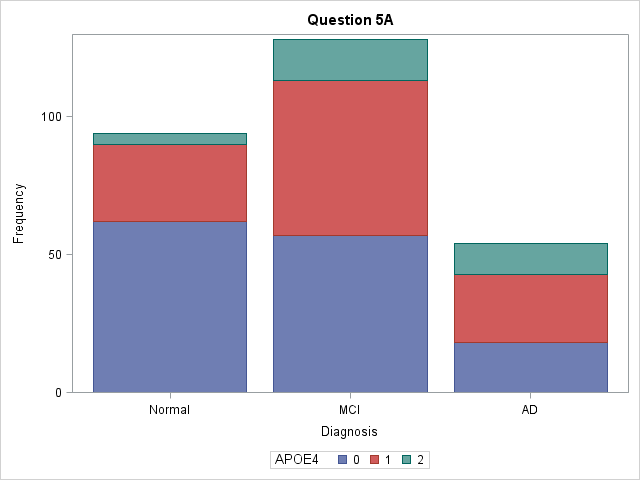
\includegraphics[width=0.45\textwidth]{Question5a1.png}
\hspace{0.1in}
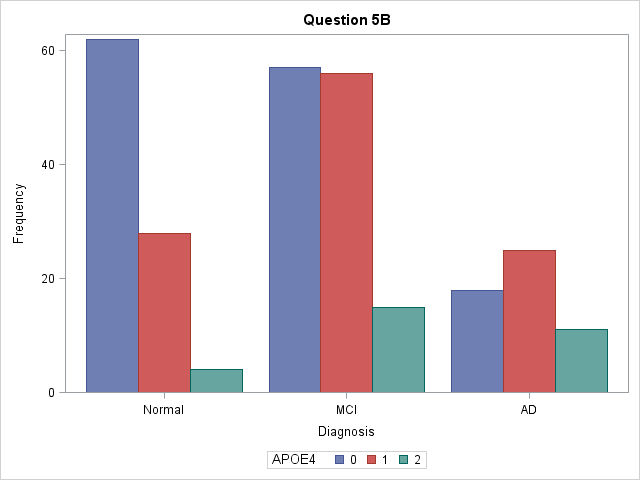
\includegraphics[width=0.45\textwidth]{Question5b1.png}\\
\vskip10pt
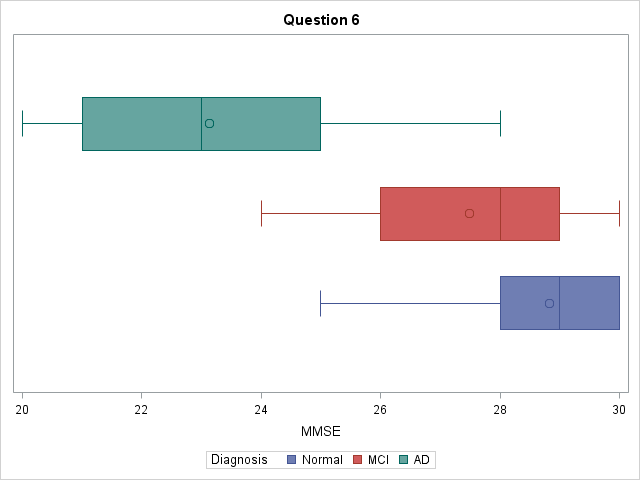
\includegraphics[width=0.45\textwidth]{Question6.png}\\
\vskip10pt
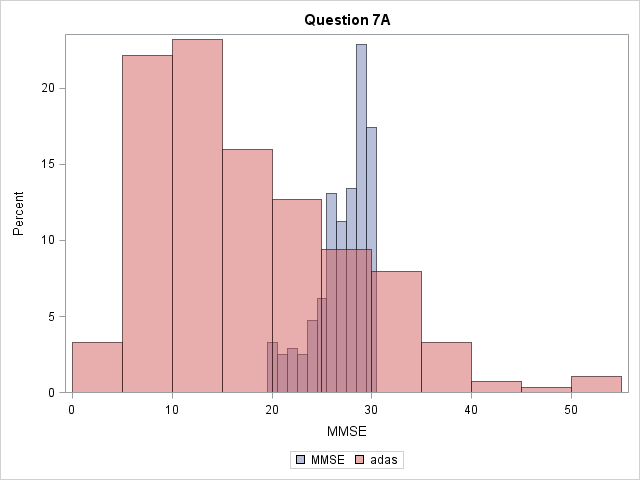
\includegraphics[width=0.45\textwidth]{Question7A.png}
\hspace{0.1in}
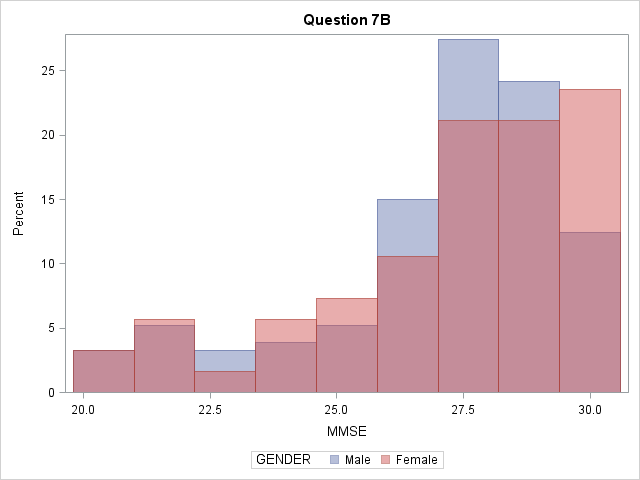
\includegraphics[width=0.45\textwidth]{Question7B.png}\\
\vskip10pt
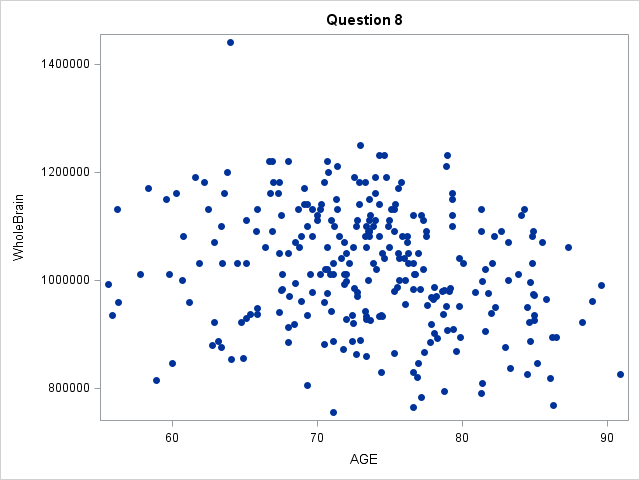
\includegraphics[width=0.45\textwidth]{Question8.png}
\hspace{0.1in}
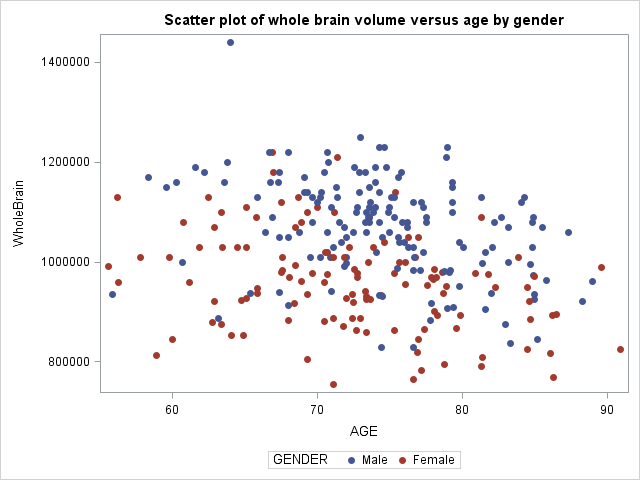
\includegraphics[width=0.45\textwidth]{Question9a.png}
\vskip10pt
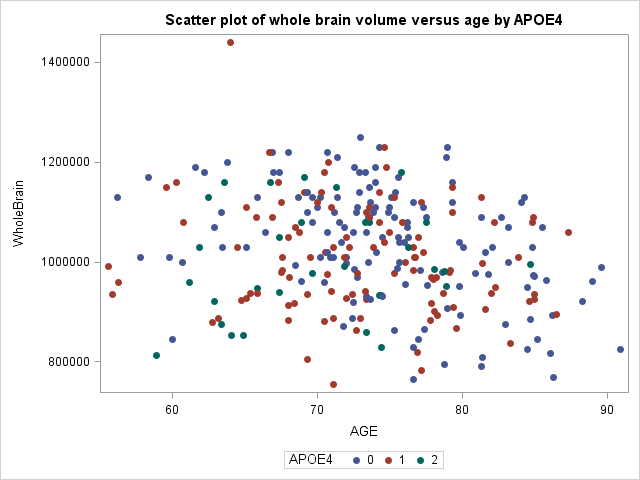
\includegraphics[width=0.45\textwidth]{Question9b.png}
\hspace{0.1in}
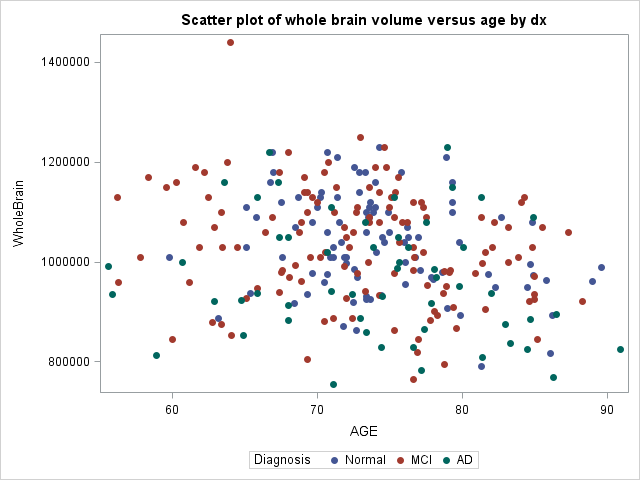
\includegraphics[width=0.45\textwidth]{Question9c.png}

\end{document}